\section{Distribution Analysis}
\label{sec:dist}

%\begin{figure}[t!]
%\begin{center}
%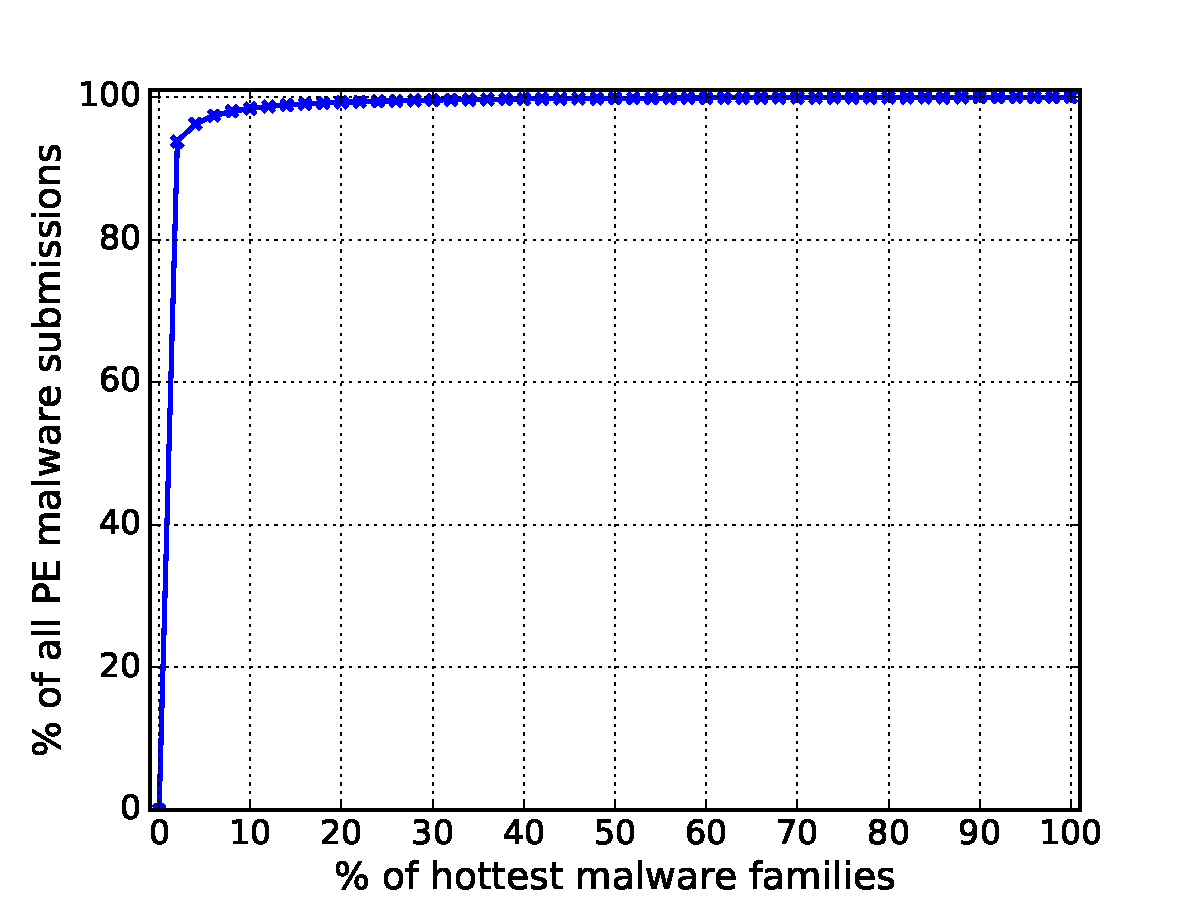
\includegraphics[width=2.5in]{figure/cum}
%\caption{Skewness of malware families appearing in November 2015.}
%\label{fig:acum}
%\end{center}
%\end{figure}

\begin{figure}[t!]
\begin{center}
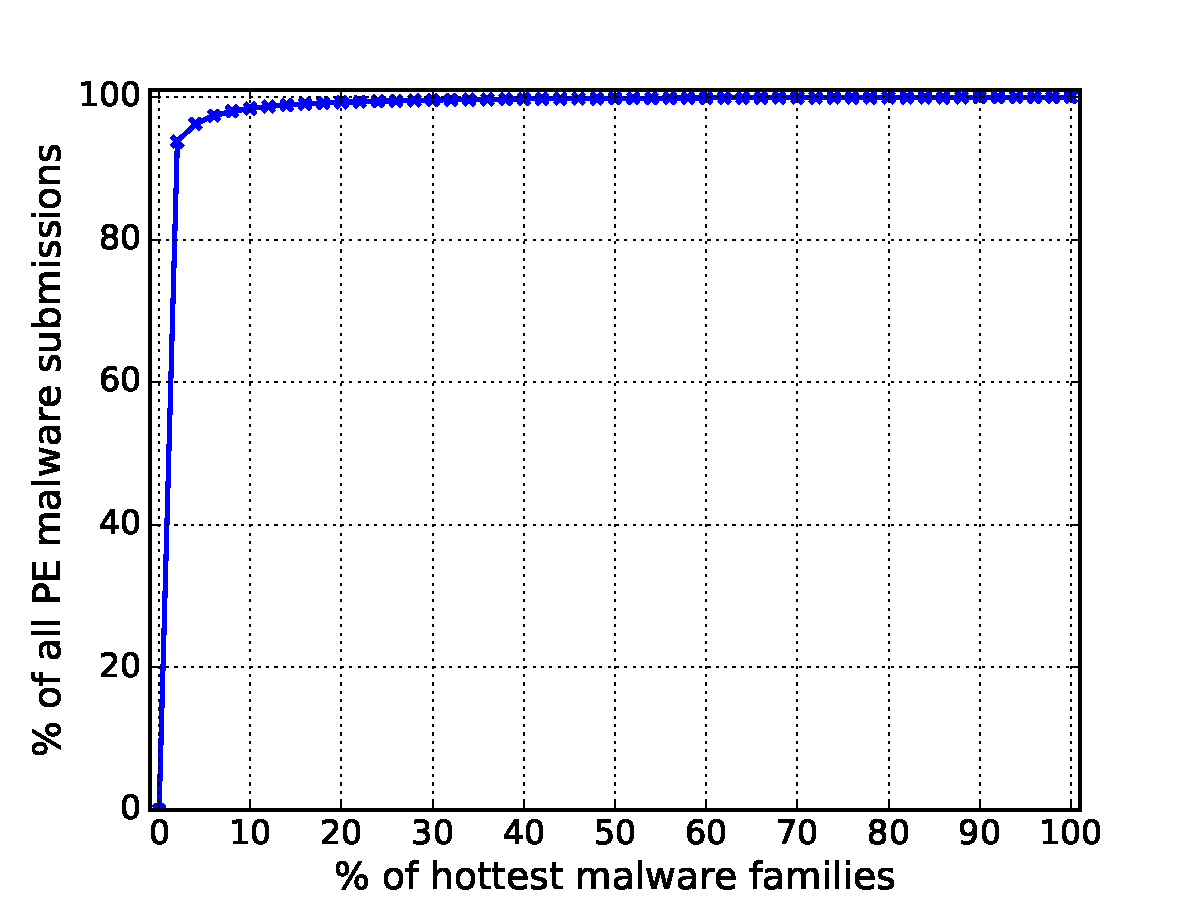
\includegraphics[width=2.5in]{figure/cum}
\mycaption{fig:acum}{Skewness of malware families appearing in November 2015.}
{Accumulation distribution of malwares in each malware family in November 2015.}
%\label{fig:acum}
\end{center}
\end{figure}






\begin{figure*}[!htb]

\minipage{0.31\textwidth}%
  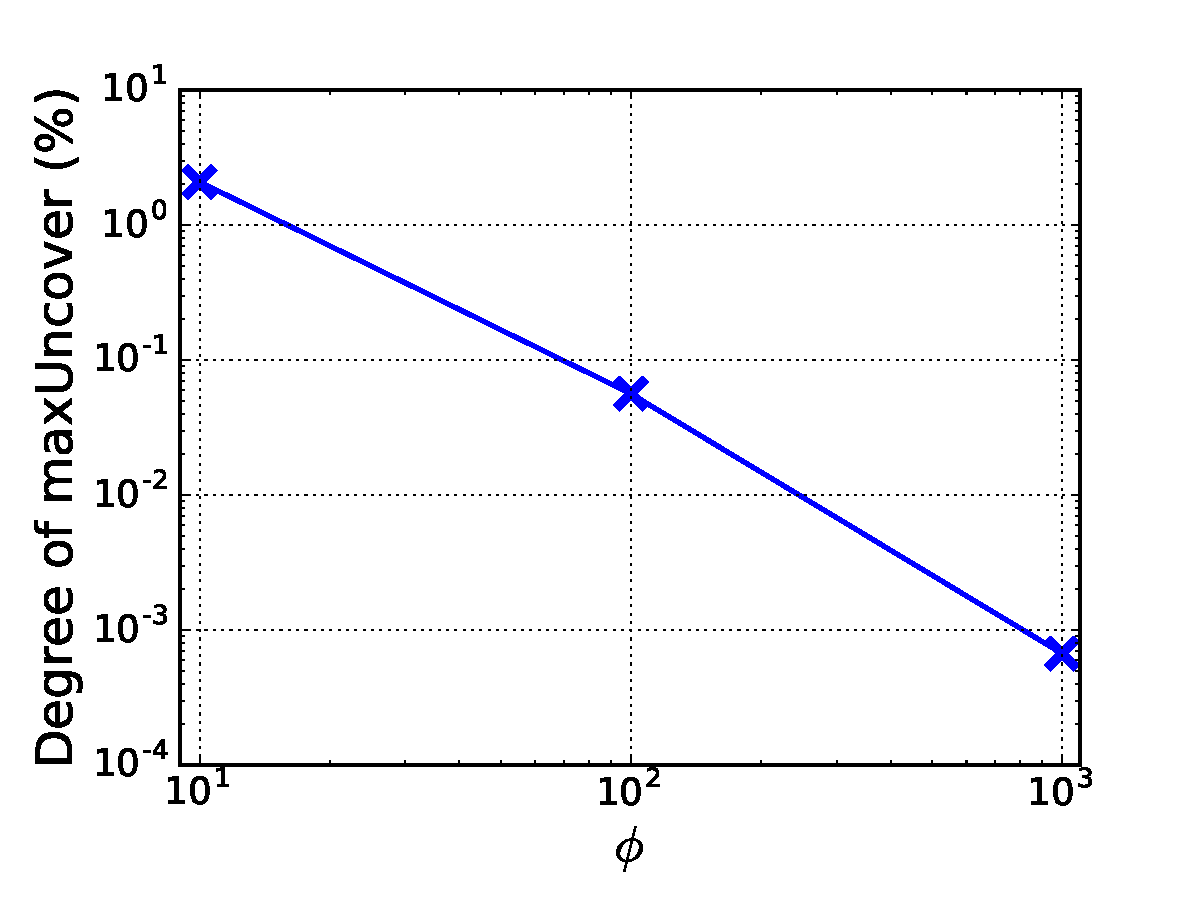
\includegraphics[width=\linewidth]{figure/maxUncover.pdf}
  \mycaption{fig:maxUncover}{Relation between $\phi$ and degree of maxUncover.}
  {
  How the degree of maxUncover changes with the change of $\phi$ from $10^{-1}$ to $10^{-3}$.
  }
  %\label{fig:aveUncover}
\endminipage\hfill
\minipage{0.31\textwidth}%
  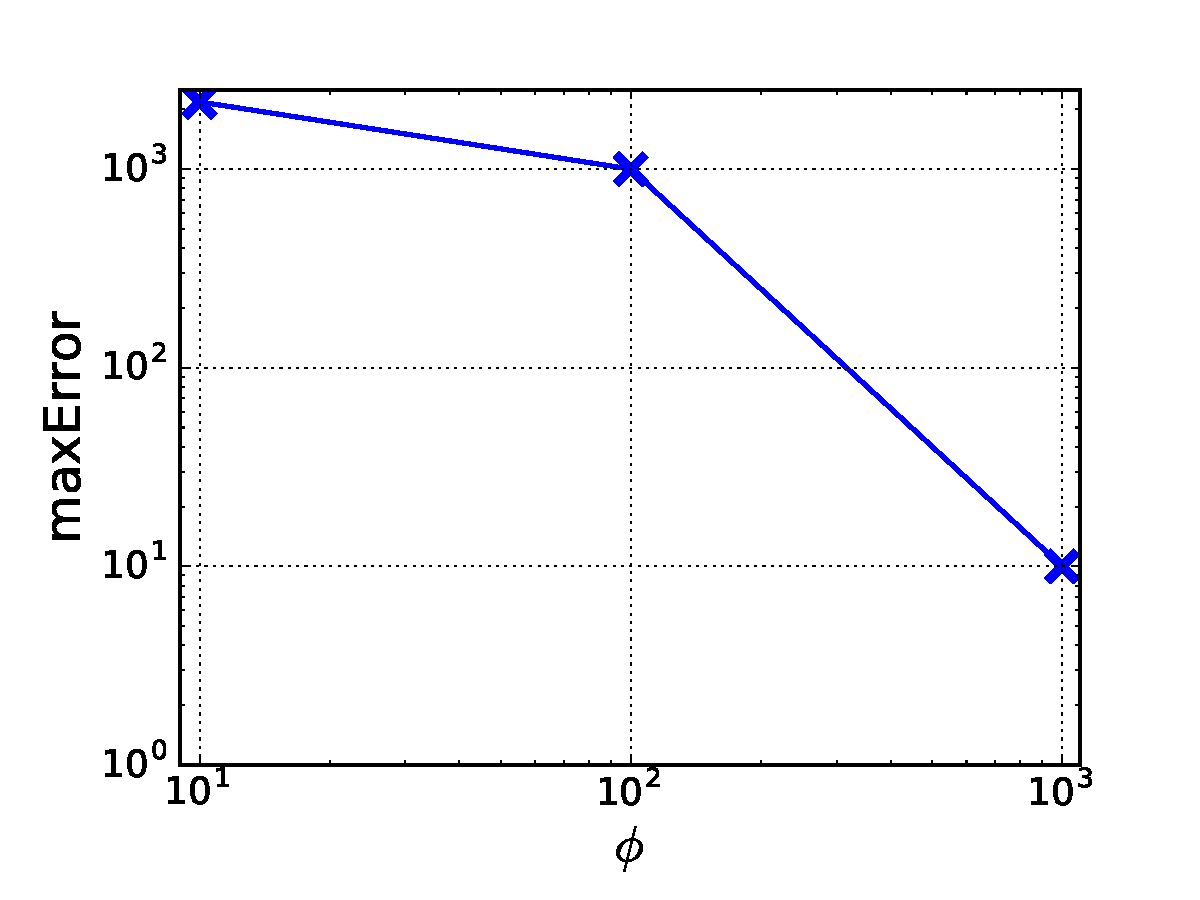
\includegraphics[width=\linewidth]{figure/maxError.pdf}
  \mycaption{fig:maxError}{Relation between $\phi$ and maxError.}
  {How maxError changes with the change of $\phi$ from $10^{-1}$ to $10^{-3}$.}
  %\caption{Relation between $\phi$ and maxError.}
  %\label{fig:maxError}

\endminipage\hfill
\minipage{0.31\textwidth}%
  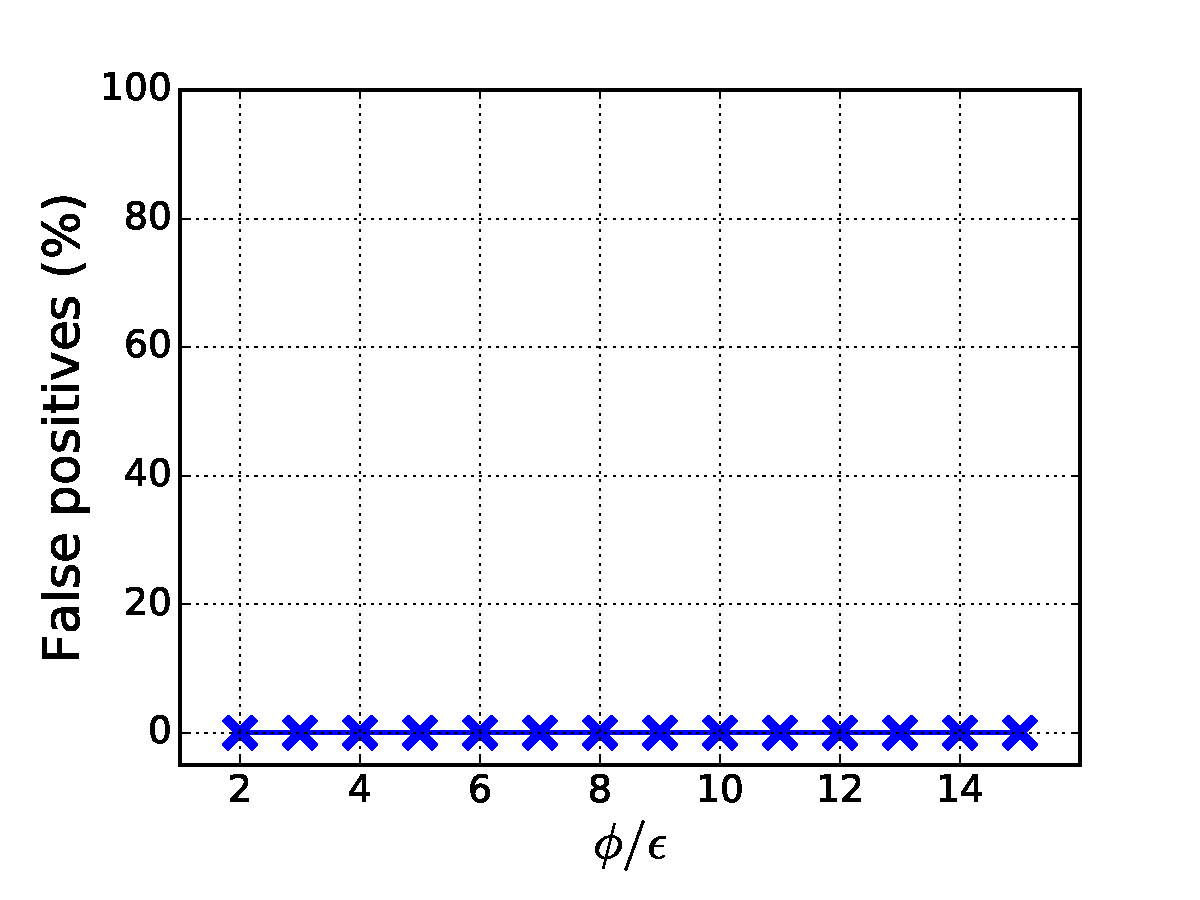
\includegraphics[width=\linewidth]{figure/fp}
  \mycaption{fig:fp}{False positives.}
{False positives in $(\phi, \epsilon)\mbox{-}HMF$ as a function of $\epsilon$. The value of $\phi$ is fixed to $10^{-2}$.
The value of $\phi/\epsilon$ changes from 2 to 15.}
  
\endminipage
\vspace{-0.1in}
\end{figure*}


\begin{figure}[t!]
\begin{center}
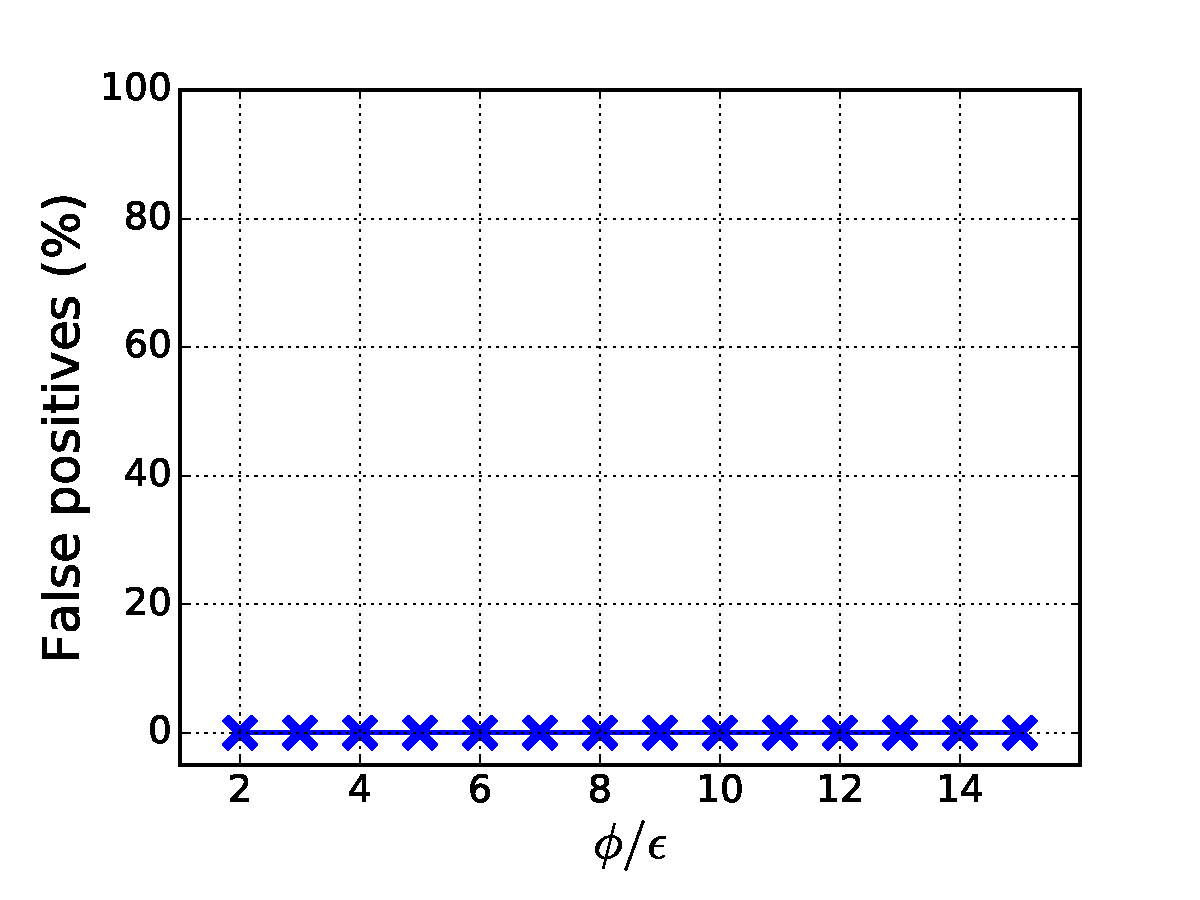
\includegraphics[width=2.0in]{figure/fp}
\mycaption{fig:fp}{False positives.}
{False positives in $(\phi, \epsilon)\mbox{-}HMF$ as a function of $\epsilon$. The value of $\phi$ is fixed to $10^{-2}$.
The value of $\phi/\epsilon$ changes from 2 to 15.}
%\label{fig:fp}
\end{center}
\end{figure}


This section presents our study on how malwares distribute in malware families. 

We first count how many malwares fall into different malware families.
As shown in Figure~\ref{fig:acum}, only a small number of malware families are hot, \ie, containing a large amount of malwares.
The distributions of malware families follow the well-known Pareto principle:  
more than 90\% of malware families take place in only 10\% of malwares. 
The distributions of malware families are highly skewed,
making it easy to precisely identify hot malware families. 

{\bf Observation 3:} {\em Distributions of malware families are highly skewed.} 

While the simple bin-counting mechanism works well on our one-month testing data, 
a total of 11311 distinct malware families, 
applying the same mechanism over a large dataset can cause significant memory space and performance overhead.

To reduce these overheads and better support online analysis of huge datasets, 
we need to seek alternative mechanisms.
The skewness of malware families indicates we can apply a frequent item mining algorithm to identify hot malware families. 

Frequent item mining algorithms take two configuration parameters, $\phi$ and $\epsilon$, where $\phi > \epsilon$. 
The goal of frequent item mining algorithms is to provide a nearly-real time analysis on massive data streams by using constant memory. 
Assuming the length of the input stream is $N$, the output of frequent item mining algorithms 
includes all items that appear more than $\lfloor \phi N \rfloor$ times 
and not include any item that appears less than  $\lfloor \epsilon N \rfloor$ times. 

The frequent item mining algorithm we use is a space-efficient algorithm~\cite{space-saving} 
proposed for streams in Internet advertising and that has already been applied in other areas, 
like mining hot calling contexts in profilers~\cite{hot-calling-context}.
Space saving algorithm tracks $M=1/\epsilon$ pairs of $(f, c)$. 
$f$ is short for malware family, and $c$ is short for counter.  
The content of these pairs represents $(\phi, \epsilon)\mbox{-}HMF$ (Hot Malware Family). 
The $M$ pairs are initialized with the first $M$ encountered malware families and their frequency. 
When a new malware submission arrives, 
if the malware family is already being monitored, 
the related counter will be increased by 1. 
And if the malware family is not being monitored, 
we will replace the malware family of the pair with the lowest counter value with the incoming malware family
and increase its counter value by 1. 
When querying HMF, 
all malware families whose counter values are larger than $\lfloor \phi N \rfloor$ will be returned. 


We implement the space saving algorithm using Python
and conduct experiments in the same system as we did in Section~\ref{sec:temporal}.
Following previous works on frequent item mining~\cite{hot-calling-context}, 
we measure the following metrics by using the malware submission data we collect:

\begin{enumerate}

\item 
Degree of \textit{overlap} is used to measure the percentage of malwares covered in $(\phi, \epsilon)\mbox{-}HMF$,
and it is defined as follows:

\begingroup\makeatletter\def\f@size{8}\check@mathfonts
$$overlap((\phi, \epsilon)\mbox{-}HMF) = \dfrac{1}{N}\sum_{f \in (\phi, \epsilon)\mbox{-}HMF}w(f)$$
\endgroup

where $w(f)$ represents the real frequency of malware family $f$.  

\item 
\textit{MaxUncover} is short for maximum frequency of uncovered malware families. 
%is used 
%to measure largest frequency of malware families not covered in $(\phi, \epsilon)\mbox{-}HMF$. 
It is defined as follows:
\begingroup\makeatletter\def\f@size{8}\check@mathfonts
$$maxUncover((\phi, \epsilon)\mbox{-}HMF) = \max_{f \notin (\phi, \epsilon)\mbox{-}HMF}w(f)/H(f)$$
\endgroup
where $H(f)$ is the maximum frequency of all malware families. 

\item 
\textit{AveUncover} is short for average frequency of uncovered malware families 
and it is defined in a manner similar to \textit{maxUncover}. 

\item 
\textit{False positives} are defined as malware families returned when querying HMF
but whose real frequencies are less than $\lfloor \phi N \rfloor$. 
Space saving algorithm is designed to guarantee that there will be no false negatives. 

\item 
\textit{MaxError} is used to measure the relative error of counter values
compared to their real frequencies.
It is defined as follows:
\begingroup\makeatletter\def\f@size{8}\check@mathfonts
$$maxError((\phi, \epsilon)\mbox{-}HMF) = \max_{f \in (\phi, \epsilon)\mbox{-}HMF} \dfrac{\left|c(f) - w(f)\right|}{w(f)}$$
\endgroup


\end{enumerate}

There are two configuration parameters in space saving algorithm: $\phi$ and $\epsilon$, 
and the number of monitored $(f, c)$ pairs is directly controlled by $\epsilon$. 
Following previous experience in applying space saving algorithm~\cite{hot-calling-context}, 
we set $\epsilon = \phi/5$ as the default, 
unless we explicitly state otherwise.  

We first evaluate how the degree of \textit{overlap} would change with the change of $\phi$. 
The degree of \textit{overlap} is used to describe how many malwares are monitored in $(\phi, \epsilon)\mbox{-}HMF$, and the larger it is, the better. 
As shown by Figure~\ref{fig:overlap}, after we change $\phi$ from 10 to 100, the degree of \textit{overlap} increases from 79.93\% to 95.48\%. 
The degree of \textit{overlap} further increases to 99.70\% after we change $\phi$ to 1000. 

We then study how maxUncover and aveUncover would change with the change of $\phi$.
Both maxUncover and aveUncover are used to describe malwares not monitored in $(\phi, \epsilon)\mbox{-}HMF$, 
and the lower they are, the better. 
As shown by Figure~\ref{fig:maxUncover} and Figure~\ref{fig:aveUncover}, 
both maxUncover and aveUncover decrease by an order as we increase the $\phi$ value by an order. 

Figure~\ref{fig:maxError} shows how \textit{maxError} changes after we change $\phi$. 
\textit{maxError} describes how precise the counters in $(\phi, \epsilon)\mbox{-}HMF$ are, 
and the lower it is, the better. \textit{maxError} drops from 2178 to 999 
after we change the value of $\phi$ from 10 to 100. 
\textit{maxError} value becomes 10 after we change the value $\phi$ to 1000. 
The large \textit{maxError} value is due to the fact that space saving algorithm 
will conservatively assume that the frequency of a new malware family is one larger than the smallest counter value of all monitored malware families. 

In the last experiment, we fix $\phi$ to $10^{-2}$ 
and change $\phi/\epsilon$ from 2 to 15 to evaluate how false positives would change. 
As shown by Figure~\ref{fig:fp}, space saving algorithm constantly reports 0 false positives in our experiments. 

